
\section{Overview}
\label{sec:overview}
	Signal will fade during the transmitting and power will loss no matter what kind of transmitter be used. As a result, we can estimate the distance between the receiver and transmitter if we know the properties of the wireless signal. Meanwhile, the phase of signal will shift when receiver get a signal, which related to their direction of arrival. In this case, out project decide to use the MUSIC algorithm and path loss to estimate direction and distance between multiple robots.
\par
	Due to the interaction of noise, one of the biggest challenges is to recover the original signal with considering white noise and Rayleigh fading noise. To easily understand the effect of these noise, the following figures are the simulation of some common signals when addictive noise is applied. Figure 4 is a sine wave without applying any noise 
\begin{figure}[ht]
	\centering
	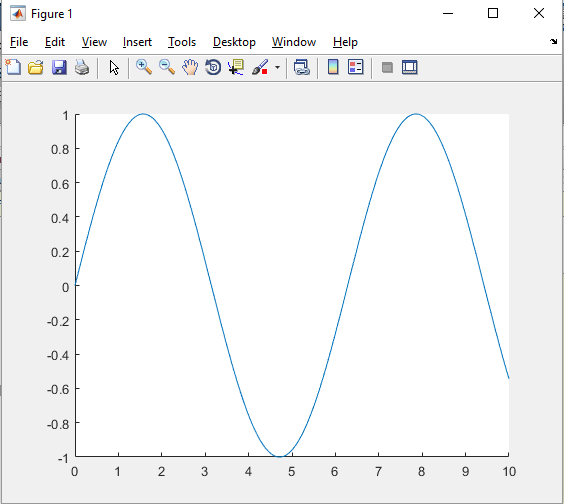
\includegraphics[width=0.4\textwidth]{noise1}
	\caption{sin waveform}
	%\label{fig1}
	\end{figure}	
\par	
Figure 5 is normal Rayleigh fading noise. \\
	\begin{figure}[ht]
	\centering
	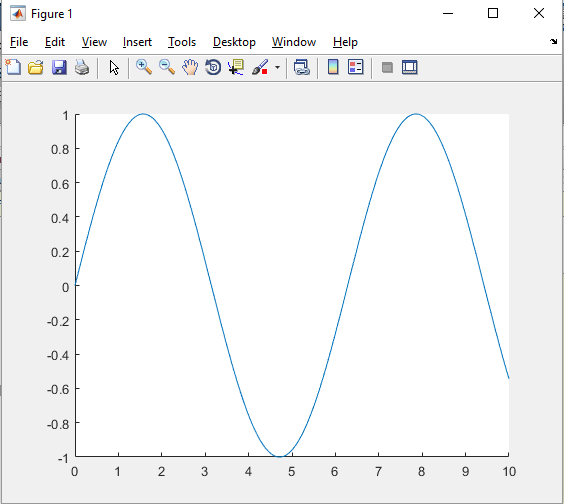
\includegraphics[width=0.4\textwidth]{noise1}
	\caption{sin waveform}
	%\label{fig1}
	\end{figure}
\par
	When we apply this noise to sine wave, the signal will look like figure 6. Rayleigh fading noise is much larger than white noise.  		

	\begin{figure}[ht]
	\centering
	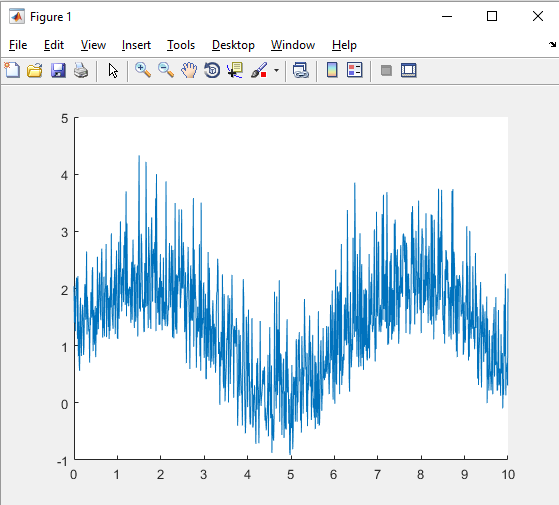
\includegraphics[width=0.4\textwidth]{noise3}
	\caption{sin waveform added with Rayleigh fading noise}
	%\label{fig1}
	\end{figure}
	
	
	
	
	\par
	To simulate our signal processing, we are going to use Matlab to model signals and apply them in simulation field, then we will integrate them with MUSIC algorithm and finally get DOA location, which will be described in detail later. 

%\begin{figure}[h]
%\centering
%\includegraphics[width=1.0\linewidth]{img/structure}
%\caption{mobility model structure}
%\label{fig1}
%\end{figure} 

